\tikzset{>=latex}
\contourlength{1.1pt}

\colorlet{mydarkblue}{blue!50!black}
\colorlet{myred}{red!65!black}
\colorlet{watercol}{blue!80!cyan!10!white}
\colorlet{darkwatercol}{blue!80!cyan!20!white}
\tikzstyle{piston}=[blue!50!black,top color=blue!30,bottom color=blue!50,middle color=blue!20,shading angle=0]
\tikzstyle{water}=[draw=mydarkblue,top color=watercol!90,bottom color=watercol!90!black,shading angle=5]
\tikzstyle{vertical water}=[water,
  top color=watercol!90!black!90,bottom color=watercol!90!black!90,middle color=watercol!80,shading angle=90]
\def\tick#1#2{\draw[thick] (#1)++(#2:0.1) --++ (#2-180:0.2)}

% PRESSURE TORRICELLI




% OPEN MANOMETER


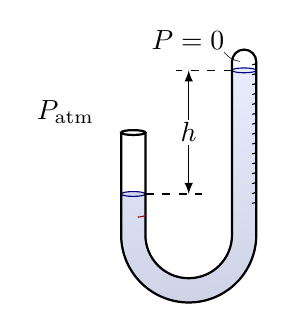
\begin{tikzpicture}
  \def\W{0.8}       % pressure box height
  \def\H{0.7}       % pressure box height
  \def\Rx{0.55}     % tube bend radius horizontal
  \def\Ry{0.2*\Rx}  % tube bend radius vertical
  \def\rx{0.28*\Rx} % tube radius horizontal
  \def\ry{0.28*\Ry} % tube radius vertical
  \def\HL{1.3}      % tube height left
  \def\HR{2.2}      % stube height right
  \def\hL{0.40*\HL} % water level height left
  \def\hR{0.95*\HR} % water level height right
  %\def\th{2.7*\H}   % tube height
  %\def\ty{0.93*\th} % tube level
  \def\N{14}
  
  % WATER + CONTAINER
  \draw[water]
    (-\Rx,\hL) --++ (0,-\hL) arc(180:360:\Rx) --++ (0,\hR) --++ (2*\rx,0) --++
    (0,-\hR) arc(360:180:\Rx+2*\rx) --++ (0,\hL);
  \draw[water]
    (-\Rx-\rx,\hL) ellipse({\rx} and {\ry})
    (\Rx+\rx,\hR) ellipse({\rx} and {\ry});
  \draw[thick]
    (-\Rx,\HL) --++ (0,-\HL) arc(180:360:\Rx) --++ (0,\HR) coordinate (T) arc(180:0:\rx)
    --++ (0,-\HR) arc(360:180:\Rx+2*\rx) --++ (0,\HL);
  \draw[thick]
    (-\Rx-\rx,\HL) ellipse({\rx} and {\ry});
  \foreach \i [evaluate={\y=(\hL+\hR)/2+0.8*\HR*(\i-\N/2)/\N;}] in {0,...,\N}{
    \draw[line cap=round] (\Rx+2*\rx+0.007,\y) arc(0:-50:{\rx} and \ry);
  }
  %\draw[line cap=round,myred] (\Rx+2*\rx+0.007,{(\hL+\hR)/2}) arc(0:-70:{\rx} and \ry);
  \draw[line cap=round,myred] (-\Rx+0.007,\hL+\hR-\HR-\rx) arc(0:-70:{\rx} and \ry);
  \node at (-\W/2-4*\rx-\Rx,\HL+1.7*\rx) {$P_\mathrm{atm}$};
  \draw[very thin,line cap=round]
    (T)++(130:\rx) node[anchor=-19,inner sep=1] {$P=0$} to[out=-50,in=170]++ (-30:1.5*\rx);
  \draw[dashed] (-\Rx,\hL) --++ (1.3*\Rx,0) (\Rx,\hR) --++ (-1.3*\Rx,0);
  \draw[<->] (0,\hL) -- (0,\hR) node[midway,fill=white,inner sep=1] {$h$};
  
\end{tikzpicture}
